% Options for packages loaded elsewhere
\PassOptionsToPackage{unicode}{hyperref}
\PassOptionsToPackage{hyphens}{url}
\PassOptionsToPackage{dvipsnames,svgnames*,x11names*}{xcolor}
%
\documentclass[
  english,
  ,man]{apa6}
\usepackage{lmodern}
\usepackage{amssymb,amsmath}
\usepackage{ifxetex,ifluatex}
\ifnum 0\ifxetex 1\fi\ifluatex 1\fi=0 % if pdftex
  \usepackage[T1]{fontenc}
  \usepackage[utf8]{inputenc}
  \usepackage{textcomp} % provide euro and other symbols
\else % if luatex or xetex
  \usepackage{unicode-math}
  \defaultfontfeatures{Scale=MatchLowercase}
  \defaultfontfeatures[\rmfamily]{Ligatures=TeX,Scale=1}
\fi
% Use upquote if available, for straight quotes in verbatim environments
\IfFileExists{upquote.sty}{\usepackage{upquote}}{}
\IfFileExists{microtype.sty}{% use microtype if available
  \usepackage[]{microtype}
  \UseMicrotypeSet[protrusion]{basicmath} % disable protrusion for tt fonts
}{}
\makeatletter
\@ifundefined{KOMAClassName}{% if non-KOMA class
  \IfFileExists{parskip.sty}{%
    \usepackage{parskip}
  }{% else
    \setlength{\parindent}{0pt}
    \setlength{\parskip}{6pt plus 2pt minus 1pt}}
}{% if KOMA class
  \KOMAoptions{parskip=half}}
\makeatother
\usepackage{xcolor}
\IfFileExists{xurl.sty}{\usepackage{xurl}}{} % add URL line breaks if available
\IfFileExists{bookmark.sty}{\usepackage{bookmark}}{\usepackage{hyperref}}
\hypersetup{
  pdftitle={Evolution of Statistical Software and Quantitative Methods},
  pdfauthor={Brandon LeBeau~\& Ariel M. Aloe},
  pdflang={en-EN},
  pdfkeywords={Research Synthesis, Statistical Software, Quantitative Methods},
  colorlinks=true,
  linkcolor=blue,
  filecolor=Maroon,
  citecolor=Blue,
  urlcolor=Blue,
  pdfcreator={LaTeX via pandoc}}
\urlstyle{same} % disable monospaced font for URLs
\usepackage{longtable,booktabs}
% Correct order of tables after \paragraph or \subparagraph
\usepackage{etoolbox}
\makeatletter
\patchcmd\longtable{\par}{\if@noskipsec\mbox{}\fi\par}{}{}
\makeatother
% Allow footnotes in longtable head/foot
\IfFileExists{footnotehyper.sty}{\usepackage{footnotehyper}}{\usepackage{footnote}}
\makesavenoteenv{longtable}
\usepackage{graphicx}
\makeatletter
\def\maxwidth{\ifdim\Gin@nat@width>\linewidth\linewidth\else\Gin@nat@width\fi}
\def\maxheight{\ifdim\Gin@nat@height>\textheight\textheight\else\Gin@nat@height\fi}
\makeatother
% Scale images if necessary, so that they will not overflow the page
% margins by default, and it is still possible to overwrite the defaults
% using explicit options in \includegraphics[width, height, ...]{}
\setkeys{Gin}{width=\maxwidth,height=\maxheight,keepaspectratio}
% Set default figure placement to htbp
\makeatletter
\def\fps@figure{htbp}
\makeatother
\setlength{\emergencystretch}{3em} % prevent overfull lines
\providecommand{\tightlist}{%
  \setlength{\itemsep}{0pt}\setlength{\parskip}{0pt}}
\setcounter{secnumdepth}{-\maxdimen} % remove section numbering
\shorttitle{Evolution Software and Methods}
\affiliation{
\vspace{0.5cm}
\textsuperscript{1} University of Iowa}
\keywords{Research Synthesis, Statistical Software, Quantitative Methods}
\usepackage{csquotes}
\usepackage{upgreek}
\captionsetup{font=singlespacing,justification=justified}

\usepackage{longtable}
\usepackage{lscape}
\usepackage{multirow}
\usepackage{tabularx}
\usepackage[flushleft]{threeparttable}
\usepackage{threeparttablex}

\newenvironment{lltable}{\begin{landscape}\begin{center}\begin{ThreePartTable}}{\end{ThreePartTable}\end{center}\end{landscape}}

\makeatletter
\newcommand\LastLTentrywidth{1em}
\newlength\longtablewidth
\setlength{\longtablewidth}{1in}
\newcommand{\getlongtablewidth}{\begingroup \ifcsname LT@\roman{LT@tables}\endcsname \global\longtablewidth=0pt \renewcommand{\LT@entry}[2]{\global\advance\longtablewidth by ##2\relax\gdef\LastLTentrywidth{##2}}\@nameuse{LT@\roman{LT@tables}} \fi \endgroup}


\DeclareDelayedFloatFlavor{ThreePartTable}{table}
\DeclareDelayedFloatFlavor{lltable}{table}
\DeclareDelayedFloatFlavor*{longtable}{table}
\makeatletter
\renewcommand{\efloat@iwrite}[1]{\immediate\expandafter\protected@write\csname efloat@post#1\endcsname{}}
\makeatother
\usepackage{tabularx}
\usepackage{pdflscape}
\ifxetex
  % Load polyglossia as late as possible: uses bidi with RTL langages (e.g. Hebrew, Arabic)
  \usepackage{polyglossia}
  \setmainlanguage[]{english}
\else
  \usepackage[shorthands=off,main=english]{babel}
\fi
\newlength{\cslhangindent}
\setlength{\cslhangindent}{1.5em}
\newenvironment{cslreferences}%
  {\setlength{\parindent}{0pt}%
  \everypar{\setlength{\hangindent}{\cslhangindent}}\ignorespaces}%
  {\par}

\title{Evolution of Statistical Software and Quantitative Methods}
\author{Brandon LeBeau\textsuperscript{1}~\& Ariel M. Aloe\textsuperscript{1}}
\date{}

\authornote{

Correspondence concerning this article should be addressed to Brandon LeBeau, Psychological and Quantitative Foundations, University of Iowa, Iowa City, IA 52245. E-mail: \href{mailto:brandon-lebeau@uiowa.edu}{\nolinkurl{brandon-lebeau@uiowa.edu}}}

\abstract{
Statistical software is the enabling tool of quantitative research and the availability and use of the software can greatly shape which methods are used by researchers. Software that is more accessible is likely to have more users and the methods implemented within the software limits the methods accessible to researchers. Open source software, (e.g.~R), has reduced these barriers by making cutting edge statistical methods available to researchers through add-on packages. This manuscript explores the evolution of statistical software within social science research using a research synthesis to establish the state of affairs. Software and statistical analysis keywords were searched in published manuscripts from high impact journals in five disciplines, Economics, Education, Political Science, Public Policy, and Sociology. Analysis was based on research synthesis methods. Implications for open science and reproducibilty are discussed.


}

\begin{document}
\maketitle

How statistical software is used in primary research studies has important implications for the reproducibility and replicability of the research (Hedges \& Schauer, 2019; Hendrick, 1990; Insitute of Education Sciences (IES), U.S. Department of Education and National Science Foundation (NSF), 2018; Peng, 2009; Schmidt, 2009; Stodden, 2012). Without knowledge of which software and version is used in the analysis, differences in results could be due to different software implementations (i.e.~different default values in estimation, different algorithms, etc), rather than specifics about the analysis (i.e.~type I error adjustments, analysis methodology, etc) (Stodden et al., 2013). To our knowledge, in the social sciences and education, no research has actively explored which software are commonly used in published research or how often research papers cite the software they use.

Software usage is only a part of the puzzle to be able to reproduce or replicate study results and has been discussed as an issue for whether studies are reproducible or not (Peng, 2009). The statistical method(s) need to be clearly articulated in how they are used, particularly in the absence of the statistical code for the analysis. Information about algorithms used for estimation (e.g.~maximum likelihood, least squares, weighted least squares, etc.), which variables are included in statistical analyses, algorithm convergence criteria, and many others are needed to ensure that reviewers and readers of the research are able to discern how the analysis proceeded. Without clear, transparent, and open statistical methods, data processing, and other data management tasks, the ability to reproduce or replicate the study drops significantly (Peng, 2009, 2011; Stodden, 2012). Concerns about fraudulent analyses and conclusions in research may also arise if the statistical code is not submitted as part of the research (Peng, 2009).

The purpose of this paper is to explore the evolution (or lack thereof) of statistical software usage, statistical methods usage, and the interaction between the two over time in the field of education. Research synthesis methods (Cooper, 2016) will be used to explore these trends over time in published articles found in five educational research journals and a total of twelve social science research journals. Social science journals outside of education spanning economics, political science, public policy, and sociology were included in the review. Journals were selected for inclusion from those in the disciplines that had strong impact factors.

\hypertarget{statistical-software-and-reproducibility}{%
\section{Statistical Software and Reproducibility}\label{statistical-software-and-reproducibility}}

Statistical software is an enabling tool to performing applied data analysis. Statistical methods that are implemented within software will increase their usage (particularly if the software is also user-friendly) by applied analysts and are likely taught more frequently in methodology courses at universities. Moreover, casual users of statistics software may not distinguish between the limitations of the models and the limitations of the software. However, the user-friendly nature of software (i.e., point and click graphical interfaces, ability to manipulate data by hand) can also severely limit the ability for research to be reproducible; a recent topic of discussion in biostatistics, medicine, and psychology (Asendorpf et al., 2013; Ioannidis, 2014; Iqbal, Wallach, Khoury, Schully, \& Ioannidis, 2016; Peng, 2009, 2011; Stodden, 2012). The replicability and reproducibility crisis has pointed the finger at statistical software more directly with a strong emphasis in some disciplines for analyses to be script (i.e., source code) based and posted with the published journal article, often described as the gold standard (Miguel et al., 2014; Peng, 2009, 2011; Stodden et al., 2013).

This idea of reproducibility has not fully entered the social science research domain, where replication has seen more focus in the literature (Asendorpf et al., 2013; Hedges \& Schauer, 2019; Hendrick, 1990; Insitute of Education Sciences (IES), U.S. Department of Education, 2018; Insitute of Education Sciences (IES), U.S. Department of Education and National Science Foundation (NSF), 2018; Makel \& Plucker, 2014; Makel, Plucker, \& Hegarty, 2012; Schmidt, 2009). There are discussions within the social science literature about ways to enhance replication which include aspects of reproducibility (Asendorpf et al., 2013; Insitute of Education Sciences (IES), U.S. Department of Education and National Science Foundation (NSF), 2018), however the focus is on enhancing replicability in which reproducibility is helpful in this regard. Reproducibility in the Educational literature is found referring to open science practices which advocate for the releasing statistical code, data, and ensuring manuscripts are able to be read openly instead of being behind paywalls (Makel, Smith, McBee, Peters, \& Miller, 2019; McBee, Makel, Peters, \& Matthews, 2018).

SPSS (IBM Corp, 2019) is likely the most common statistical software program used in many social science research domains, particularly education. Although SPSS has many common and advanced statistical techniques and it is possible to have a reproducible analysis, the default behavior within SPSS is not script based and can create bad habits. For example, editing raw data directly in the graphical user interface, running analyses without saving a script, creation of variables without syntax, or marking values as missing or not possible in the variable view window. Statistical software that is primarily command line, programs such as R (R Core Team, 2019), Python (Van Rossum \& Drake Jr, 1995), SAS (SAS Institute, 2017), or Stata (StataCorp, 2019), offer easier reproducible frameworks as all data manipulations or analyses are saved in scripts that can be re-ran in the future. A data script can be thought of as a cockpit flight recorder in which every single step that was done to the original data going from data collection to final tables and figures were script based. Under a reproducible framework, the raw data are never altered directly, they should always be altered programmatically through a script. This keeps a log of the data manipulations that happened in the data analysis cycle. For example, R, Python, and Stata have packages or functionality that aid in the ability to create living data documents that contain text and analysis code within a single document (see Allaire et al., 2017; Kluyver et al., 2016; StataCorp, 2019; Xie, 2015, 2017).

The reproducible analysis framework has many advantages, including a transparent analysis process that could be validated (i.e.~reproduced) by others, including reviewers, journal editors, students etc. Unfortunately, the current publishing environment has many barriers that limit the reproducibility of research. First, applied researchers may not be users of primarily command line or script based statistical software. This limits the ability to create a reproducible analysis from the start. Secondly, researchers are not incentivized to conduct a reproducible analysis. In particular, the publish or perish aspect of tenure track positions limits the sharing of statistical code partly due to the increased chance of criticism upon evaluation of the code used for the analysis. Finally, many journals and even the American Psychological Association (APA) publication manual (American Psychological Association, 2010, p. 210) states that common software or programming languages need not be cited. This could even be interpreted by some as not needing to mention the software used in the analysis. Unfortunately, if the software used for a data analysis is not reported, the ability to recreate the analysis may decrease due to differences in estimation, handling of missing data, or other software specific default settings.

This paper aims to explore the state of affairs in statistical software usage in education and the social sciences. Particular attention will be made to which software is currently being used in published educational research as well as how this has changed over the last twenty years. Secondly, this paper also aims to explore how frequently open-source software tools are used and to explore evidence of reproducible analysis framework being implemented. Finally, comparisons of educational research journal trends to other social science disciplines will be explored. These aims will be explored using research synthesis methods.

\hypertarget{statistical-software-usage}{%
\section{Statistical Software Usage}\label{statistical-software-usage}}

Research on the usage of statistical software has rarely been undertaken. Muenchen (2017) has explored the popularity of data science software through job advertisements, scholarly articles, and other metrics. This exploration has shown that job advertisements for R and Python have increased between 2012 and 2017, but job advertisements for SAS have stayed relatively steady over this time frame based on data from Indeed's job trends tool. The number of scholarly articles, tracked through a Google Scholar search, that mention research software was also explored between 1995 and 2016 was also explored by Muenchen (2017). The data show that SPSS has dominated between the years 2000 and 2010, but since 2010 has steadily decreased although still remains the most popular mentioned software tool. SAS has been second for most of this time frame and has followed a similar trajectory as SPSS. Recently, R has passed SAS in how often it is used in 2016. Stata has also shown strong increases as well, but not quite as steep an increase as R has shown.

The current study differs from the analysis conducted by Muenchen (2017) in key ways. First, the current analysis focuses on educational and social science research, which is narrowed compared to the analysis conducted by Muenchen (2017). Secondly, the current study explores statistical methods used and the interaction between statistical methods and software usage, an area not explored by Muenchen (2017). Finally, through the methodology by Muenchen (2017), it is not directly possible to explore how many studies are not mentioning statistical software, but still mentioning statistical methods. Statistical software implementation has implications for the reproducibility and replicability of the analysis and is a focus of this research.

\hypertarget{statistical-methods-usage}{%
\section{Statistical Methods Usage}\label{statistical-methods-usage}}

Exploration of which statistical methods are being used in published research has also rarely been explored. One study by Tatman (2015) explored the usage of statistical methods in linguistics. A total of 348 articles were extracted from the most recent issue of a variety of linguistics journals. Of these 348 articles, about 65\% of the articles listed at least one of the statistical methods coded. Most of the articles that listed a statistical method only listed a single method, but a few articles had up to 10 methods listed. The most popular inferential methods found were analysis of variance, t-tests, correlations, and Chi-Square analyses.

To our knowledge, no other study has undertaken the synthesis of software usage, statistical methods usage, or the interaction between the two. This study aims to fill this gap and explore the following research questions.

\hypertarget{research-questions}{%
\subsection{Research Questions}\label{research-questions}}

\begin{enumerate}
\def\labelenumi{\arabic{enumi}.}
\tightlist
\item
  Has statistical software usage shifted over time in published educational and social science research?

  \begin{itemize}
  \tightlist
  \item
    If there is evidence of a shift, is there evidence this shift differs based on quantitative method or journal?
  \end{itemize}
\item
  How often does published research cite statistical software?

  \begin{itemize}
  \tightlist
  \item
    Has this changed over time and across journals?
  \end{itemize}
\item
  How often are open-source statistical software tools used?

  \begin{itemize}
  \tightlist
  \item
    Is there evidence of reproducible analyses being employed?
  \end{itemize}
\item
  Does the research journal discipline impact the trends explored in the first three research questions?
\end{enumerate}

\hypertarget{methods}{%
\section{Methods}\label{methods}}

Research synthesis methods (Cooper, 2016) will be used to explore the evolution of statistical software and quantitative methods in social science research. More specifically, the statistical software used for the analysis will be coded as well as the quantitative method(s) used (i.e.~linear regression, hierarchical linear model, etc.). Additional meta data will also be coded including, journal, article title, author information, article keywords, year published, and any mention of supplementary materials. This information will be used to explore descriptive trends in the data over time, by journals, and methods.

The research synthesis will gather data from a handful of education journals that primarily publish empirical data analysis. The search will not include journals that the primary focus is methodological, the use of software in these journals would likely be a different population than those that are data analytic in nature. Table \ref{tab:journals} shows the journals selected for inclusion by discipline and including the journal abbreviation that will be used primarily in reporting the study results.

\begin{table}[!h]

\caption{\label{tab:journals}Discipline and journal name of those included in the research synthesis.}
\centering
\begin{tabular}[t]{lll}
\toprule
Discipline & Journal & Journal Abbreviation\\
\midrule
Economics & American Economic Journal & AEJ\\
Economics & Educational Evaluation and Policy Analysis & EJ\\
Education & American Educational Research Journal & AERJ\\
Education & Economic Journal & EEPA\\
Education & Educational Researcher & ER\\
\addlinespace
Education & Higher Education & HE\\
Education & Journal of Experimental Education & JEE\\
Political Science & American Journal of Political Science & AJPS\\
Political Science & Journal of Public Policy & PSQ\\
Public Policy & Political Science Quarterly & PPA\\
\addlinespace
Public Policy & Public Policy Administration & JPP\\
Sociology & Sociology of Education & SE\\
\bottomrule
\end{tabular}
\end{table}

\hypertarget{data-and-software}{%
\subsection{Data and Software}\label{data-and-software}}

All journal articles published between 1995 through the middle of 2018 were organized into EndNote. The citation information was obtained using the Web of Knowledge online tool. Once the citations were added to EndNote, the find pdf feature was used to gather the published documents from each journal. This pdf database was searched using the \emph{pdfsearch} R package (LeBeau, 2018; R Core Team, 2019). This package allows for keyword searching directly within pdf documents. The package also has the benefit of converting lines of text read in from PDF files to sentences. This procedure also works for multicolumn PDF documents, which considers the natural reading flow of the text in converting the lines to sentences. These text manipulation procedures of the package can help to ensure that the context of the sentence is maintained, rather than a line of text being a part of a sentence or multiple sentences. The pdfsearch package also returns the line number in the document and the full sentence that the keyword result was found. This can allow one to hone in on where the keyword was found within the research document. The results keyword search results obtained from pdfsearch will be the primary data collection method. The software keywords searched for can be seen in Table \ref{tab:searchwords}. Table \ref{tab:searchwords} also shows keywords to be used to search for statistical analysis and estimation methods.

Additional metadata obtained from journal articles will be obtained and combined with the keyword searching data. This metadata will contain information such as, year of publication, publication keywords, author information, and other article metadata obtained from EndNote. The citation information was converted to a bibtex file and the \emph{bib2df} package (Ottolinger, 2018) was used to parse the bibtex fields to collect the metadata. These data will be used to further enhance the keyword search data obtained from the \emph{pdfsearch} package and the subsequent analyses discussed in the next section.

\begin{table}
\captionof{table}{Search keywords used in search of published journal documents.}
\label{tab:searchwords}
\begin{tabularx}{\linewidth}{llX}

\toprule
Search & Group & Keywords \\
\midrule 

\multirow{9}{*}{Software} & SPSS            & SPSS Statistics, SPSS Modeler, SPSS \\
                          & R               & R-project, R Project, CRAN, R core team, R software, RStudio \\
                          & SAS             & SAS Institute, SAS, JMP  \\
                          & STATA           & STATA          \\
                          & Python          & Python                  \\
                          & Other           & MATLAB, Statistica , Statsoft, Java, Hadoop, Minitab, Systat, Tableau, Scala, Julia, Azure Machine Learning \\
                          & HLM             & HLM[0-9], HLM [0-9]                            \\
                          & IRT             & BILOG, BILOG-MG, Multilog, PARSCALE, IRT Pro        \\
                          & Latent Variable & Mplus, LISREL, AMOS   \\
\midrule

\multirow{7}{*}{Statistical analyses} & ANOVA           & Analysis of Variance, ANOVA, ANCOVA, Analysis of Covariance, multivariate analysis of variance, MANOVA, repeated measures analysis of variance, RMANOVA, RM-ANOVA                                                                                                                                                               \\
                                    & HLM             & HLM, Hierarchical Linear Model, Linear Mixed Model, LMM, Multilevel Model, Multi-level Model                                                                                                                                                                                                                                    \\
                                    & Latent Variable & item response theory, IRT, confirmatory factor analysis, CFA, exploratory factor analysis, EFA, latent variable modeling, structural equation modeling, SEM                                                                                                                                                                     \\
                                    & t-test          & one sample t-test, one-sample t-test, two sample t-test, two-sample t-test, dependent samples t-test, dependent-sample t-test                                                                                                                                                                                                   \\
                                    & Regression      & Regression, multiple regression, linear regression, multiple linear regression, nonlinear regression, non-linear regression, logistic regression, ordinal regression, multinomial logistic regression, multinomial regression, generalized additive models, GAM, general(ized)? linear model, general(ized)? linear mixed model \\
                                    & Growth          & growth model, latent growth model, LGM                                                                                                                                                                                                                                                                                          \\
                                    & Other           & cluster analysis, hierarchical cluster analysis, propensity score matching, propensity score analysis, meta analysis, meta-analysis, nonparametric analysis, chi-square( analysis)?                                                                                                                                             \\
\bottomrule

\end{tabularx}
\end{table}

\hypertarget{analysis}{%
\subsection{Analysis}\label{analysis}}

Descriptive analyses will be performed on the research synthesis data obtained from keyword searching performed with the \emph{pdfsearch} package. Initial exploration will focus on software and statistical analyses separately. Subsequent descriptive analyses will be performed to explore if there are any interactions between software and statistical analyses used in published research. All of these analyses will be performed over time to explore trends in software and statistical analysis usage and citation rates. Figures will be the primary analysis methods and will be created in R using the ggplot2 package (Wickham, 2016).

The journal and the discipline of the journal will be used to explore differences across journals and disciplines. An in depth exploration of the education domain will be pursued to see how software and statistical methods have evolved within published research in education.

\hypertarget{limitations}{%
\subsubsection{Limitations}\label{limitations}}

The sample of journals obtained for inclusion may bias the results. The focus on this search was journals that are known broadly by each field and had strong impact factors. Impact factors are only one of many potential metrics that could have been explored. In addition, we did not consider open access journals which have become more prevalent and have become a larger part of the publishing landscape. The analysis also relies on keyword searching and the keywords searched need to match in the document exactly. This may result in the under-representing of terms when different spellings were used that were not included in the keyword search. The software keyword searches may also be biased by two factors. First, the American Psychological Association (APA) publication manual specifically mentions that common statistical software does not need to be cited. Secondly, those who are open-source software developers or use open-source software regularly may be more likely to cite the open-source software (e.g., R). The impacts of these factors are unknown however in the current literature.

\hypertarget{results}{%
\section{Results}\label{results}}

The number and percentage of PDFs obtained from EndNote is shown in Table \ref{tab:setup}. Overall, just over 10,012 journal articles were obtained out of 13,563, about a 74\% obtained article rate. These rates differed across journals however. Many of the journals had a high success rate of obtaining the PDF for the published studies, however some were problematic. For example, JPP and EEPA were both under 50\% of PDFs obtained and AJPS, EJ, and SE were all just over 50\%. The PDFs that were not obtained were attempted to be obtained over multiple occasions over a six month period, with no additional PDFs obtained between the last two attempts. There were also differences across disciplines, with education having higher success rates compared to political science or sociology.

Figure \ref{fig:pdf-time} shows the percentage of PDFs obtained by year and journal and highlights some noticeable trends. There are periods of time for specific journals that all the PDFs are obtained. For example, AJPS, EEPA, EJ, and SE have periods from 1995 to just after 2000 where most of the PDFs were not obtained. These ranges are portions of time in which our University does not have digital access to these journals, therefore this missing data is expected due to how EndNote obtains the PDF documents (i.e., the manuscript needs to be open access or our University must subscribe to the journal for access). For periods where our University has access to the journal, the success rate was very high, almost uniformly 100\%, but there were a small number of articles that were still not obtained.

\begin{table}[!h]

\caption{\label{tab:setup}EndNote success rate of obtaining article PDf by discipline and journal.}
\centering
\begin{threeparttable}
\begin{tabular}[t]{llrrr}
\toprule
Discipline & Journal & Number of PDFs & Total Possible Articles & Percent PDFs Obtained\\
\midrule
Economics & AEJ & 363 & 364 & 99.7\\
Economics & EJ & 1829 & 3376 & 54.2\\
Education & AERJ & 444 & 444 & 100.0\\
Education & EEPA & 188 & 405 & 46.4\\
Education & ER & 742 & 794 & 93.5\\
\addlinespace
Education & HE & 1914 & 1914 & 100.0\\
Education & JEE & 517 & 525 & 98.5\\
Political Science & AJPS & 922 & 1436 & 64.2\\
Political Science & PSQ & 2722 & 3589 & 75.8\\
Public Policy & PPA & 83 & 83 & 100.0\\
\addlinespace
Public Policy & JPP & 27 & 180 & 15.0\\
Sociology & SE & 261 & 453 & 57.6\\
\hline
Total &  & 10012 & 13563 & 73.8\\
\bottomrule
\end{tabular}
\begin{tablenotes}
\item \textit{Note: } 
\item AEJ = American Economic Journal; AERJ = American Educational Research Journal; AJPS = American Journal of Political Science; EJ = Economic Journal; EEPA = Educational Evaluation and Policy Analysis; ER = Educational Researcher; HE = Higher Education; JEE = Journal of Experimental Education; JPP = Journal of Public Policy; PSQ = Political Science Quarterly; PPA = Public Policy Administration; SE = Sociology of Education
\end{tablenotes}
\end{threeparttable}
\end{table}

\begin{figure}
\centering
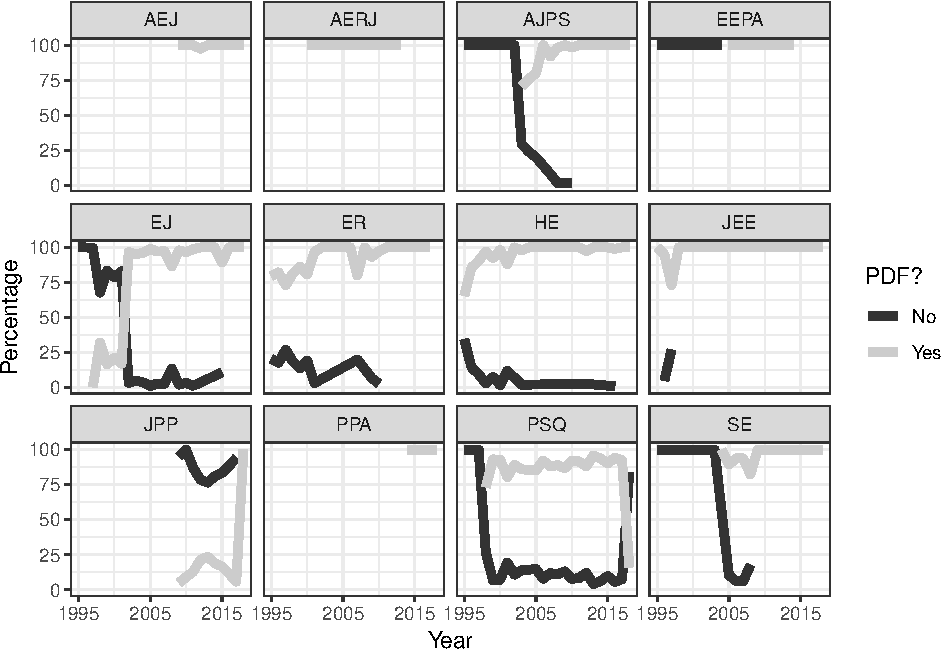
\includegraphics{software_files/figure-latex/pdf-time-1.pdf}
\caption{\label{fig:pdf-time}Number of PDFs obtained by journal and year.}
\end{figure}

Using the obtained PDFs, keyword searching was performed for the software and statistical analysis keywords. Figure \ref{fig:count-software} shows the percentage of articles from each journal with at least one match for software and analysis keywords. The figure shows that software keywords are much less likely to be found within the obtained PDFs compared to the statistical analysis keywords. The largest percentage of published articles to contain at least one matching software keyword was in JEE, about 50\%. Most of the other journals had 25\% or less of the articles mentioning one of the software keywords, with none of the obtained articles in JPP mentioning a software keyword. Analysis keywords on the other hand were much more prevalent and the journals fall into two broad groups. One group, JEE, EEPA, AEJ, AJPS, SE, and EJ have more than 50\% of the obtained articles mentioning at least one of the analysis keywords and the remaining journals being less than 50\%. The articles in the latter group, with the exception of AERJ, were closer to 25\% or fewer.

\begin{figure}
\centering
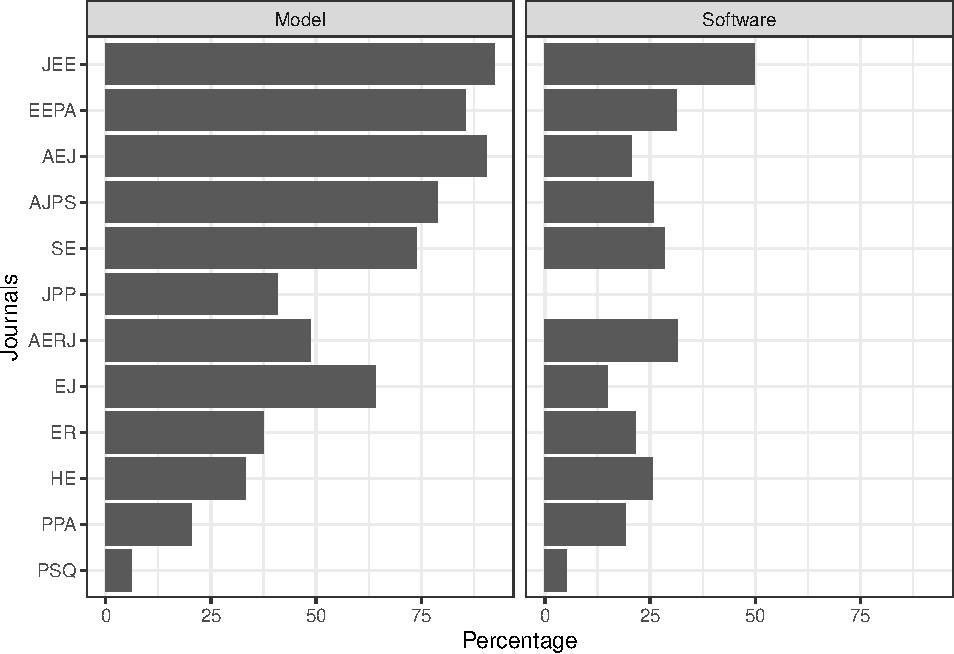
\includegraphics{software_files/figure-latex/count-software-1.pdf}
\caption{\label{fig:count-software}Number of articles with at least one model or software keyword match by journals.}
\end{figure}

\hypertarget{impact-of-research-discipline}{%
\subsection{Impact of Research Discipline}\label{impact-of-research-discipline}}

The software keyword search results show that across disciplines, R was the most likely keyword to be found, except for sociology where SAS was found slightly more often than R (Figure \ref{fig:discipline-software}). Although R was the most often keyword found in most disciplines, the percentage of studies mentioning R across the disciplines was less than 15\%, as represented in education, but more frequently was found less than 10\% of the time. Outside of sociology, which had two software keywords found more than 10\% of the time (R and SAS); for all of the other disciplines, R was found over twice the rate of other software systems.

SPSS and SAS showed up more than 5\% of the time in education, much higher rates for these software keywords compared to other disciplines. These represent, together with R, three of the four or five primary general statistical analysis software. All other specialty software was found less than 5\% of the time. In education, structural equation modeling software, AMOS, Mplus, and LISREL, had the highest keyword searches found of the specialty software. These three software programs were found much less frequently in other disciplines, except for AMOS in economics and sociology.

The data presented in Figure \ref{fig:discipline-software} may contain published manuscripts that mention more than one software keyword in a single manuscript. For instance, manuscripts that had software keywords found had on average 1.08 keywords found (range 1 to 3) for the economics discipline. Compare this to 1.67 keywords found (range 1 to 7) for the education discipline. This means, that although it looks like education has more instances of citing software in published research, there is evidence to suggest that there are a few papers in education citing multiple software keywords which is likely inflating the keyword percentage in education.

When exploring unique published research articles to calculate the proportion in each discipline that resulted in a software keyword found, sociology has evidence of citing software more frequently than other disciplines. Sociology had about 28\% of the articles found to contain at least one software keyword. After sociology, education has 21\%, public policy had 19\%, economics had 16\%, and political science was just under 10\%. Overall, these rates show that software citation varied by discipline, but has significant room for improvement.

\begin{figure}
\centering
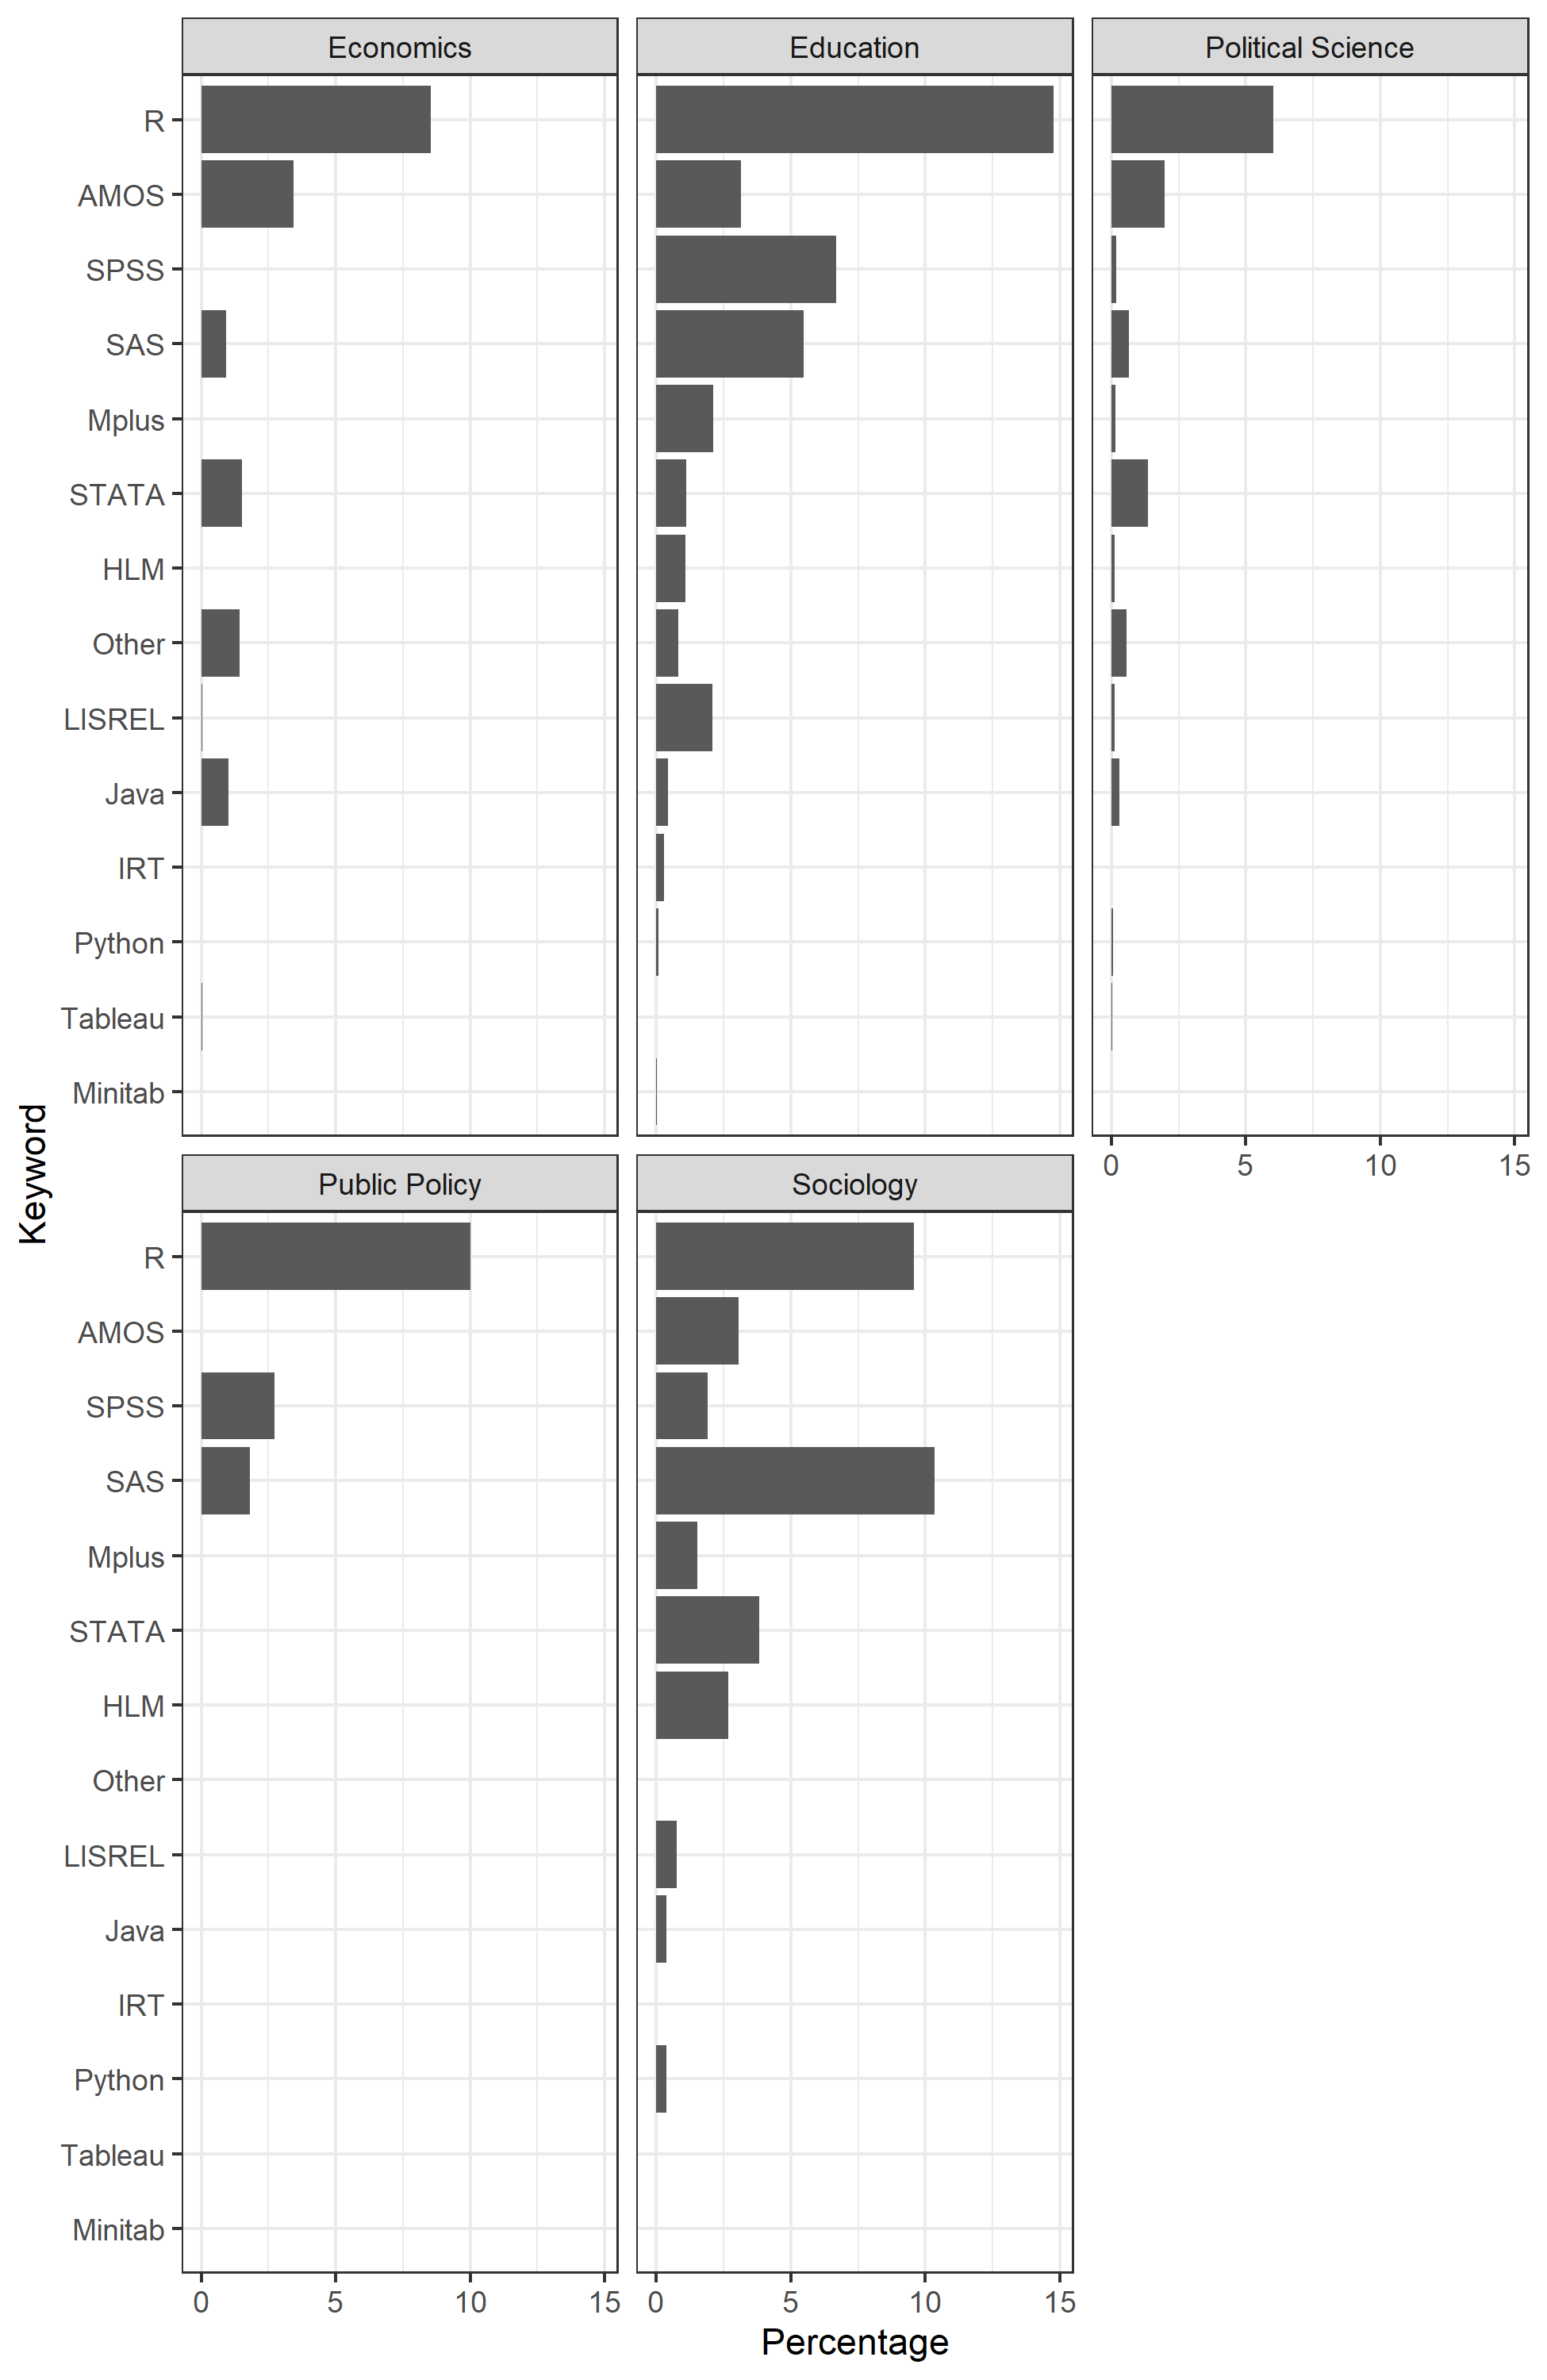
\includegraphics{software_files/figure-latex/discipline-software-1.pdf}
\caption{\label{fig:discipline-software}Counts of statistical software by journal discipline}
\end{figure}

Compared to the software keywords, statistical analysis keywords were much higher across all of the disciplines, but most notably for sociology and economics (Figure \ref{fig:model-discipline}). For economics and sociology, over 60\% of the studies mentioned linear model at least once. Sociology also had linear mixed model and logistic regression keywords show up frequently (about 20\% and 30\% respectively), where as growth was the next highest keyword for economics, but was mentioned in less than 10\% of the articles. The highest percentage in the other disciplines hovered around 20\% and was also the linear model keyword. Within education, meta-analysis and ANOVA were the next most frequent with rates around 15\%.

Similar to the results of the software keywords, the analysis keyword results may contain more than one in a single published article. For example, education had on average 3.36 analysis keywords found per published article (ranging from 1 to 12), however economics had on average 1.38 analysis keywords found per published article (ranging from 1 to 4). The other disciplines ranged between education and economics, with sociology having 2.39 on average.

Exploring the proportion of articles that cited at least one of the analysis keywords showed that sociology had the highest percentage, with 74\% of the articles found having at least one analysis keyword. Economics was the second highest about 59\%, followed by education at 27\%, public policy with 26\%, and political science with 23\%. Although 100\% analysis keyword rate found within each discipline would be unlikely, there is evidence of variation across disciplines. The extent to which this being due to some disciplines not citing the analysis method or due to other factors, such as some disciplines having more opinion pieces or qualitative analyses is not known.

\begin{figure}
\centering
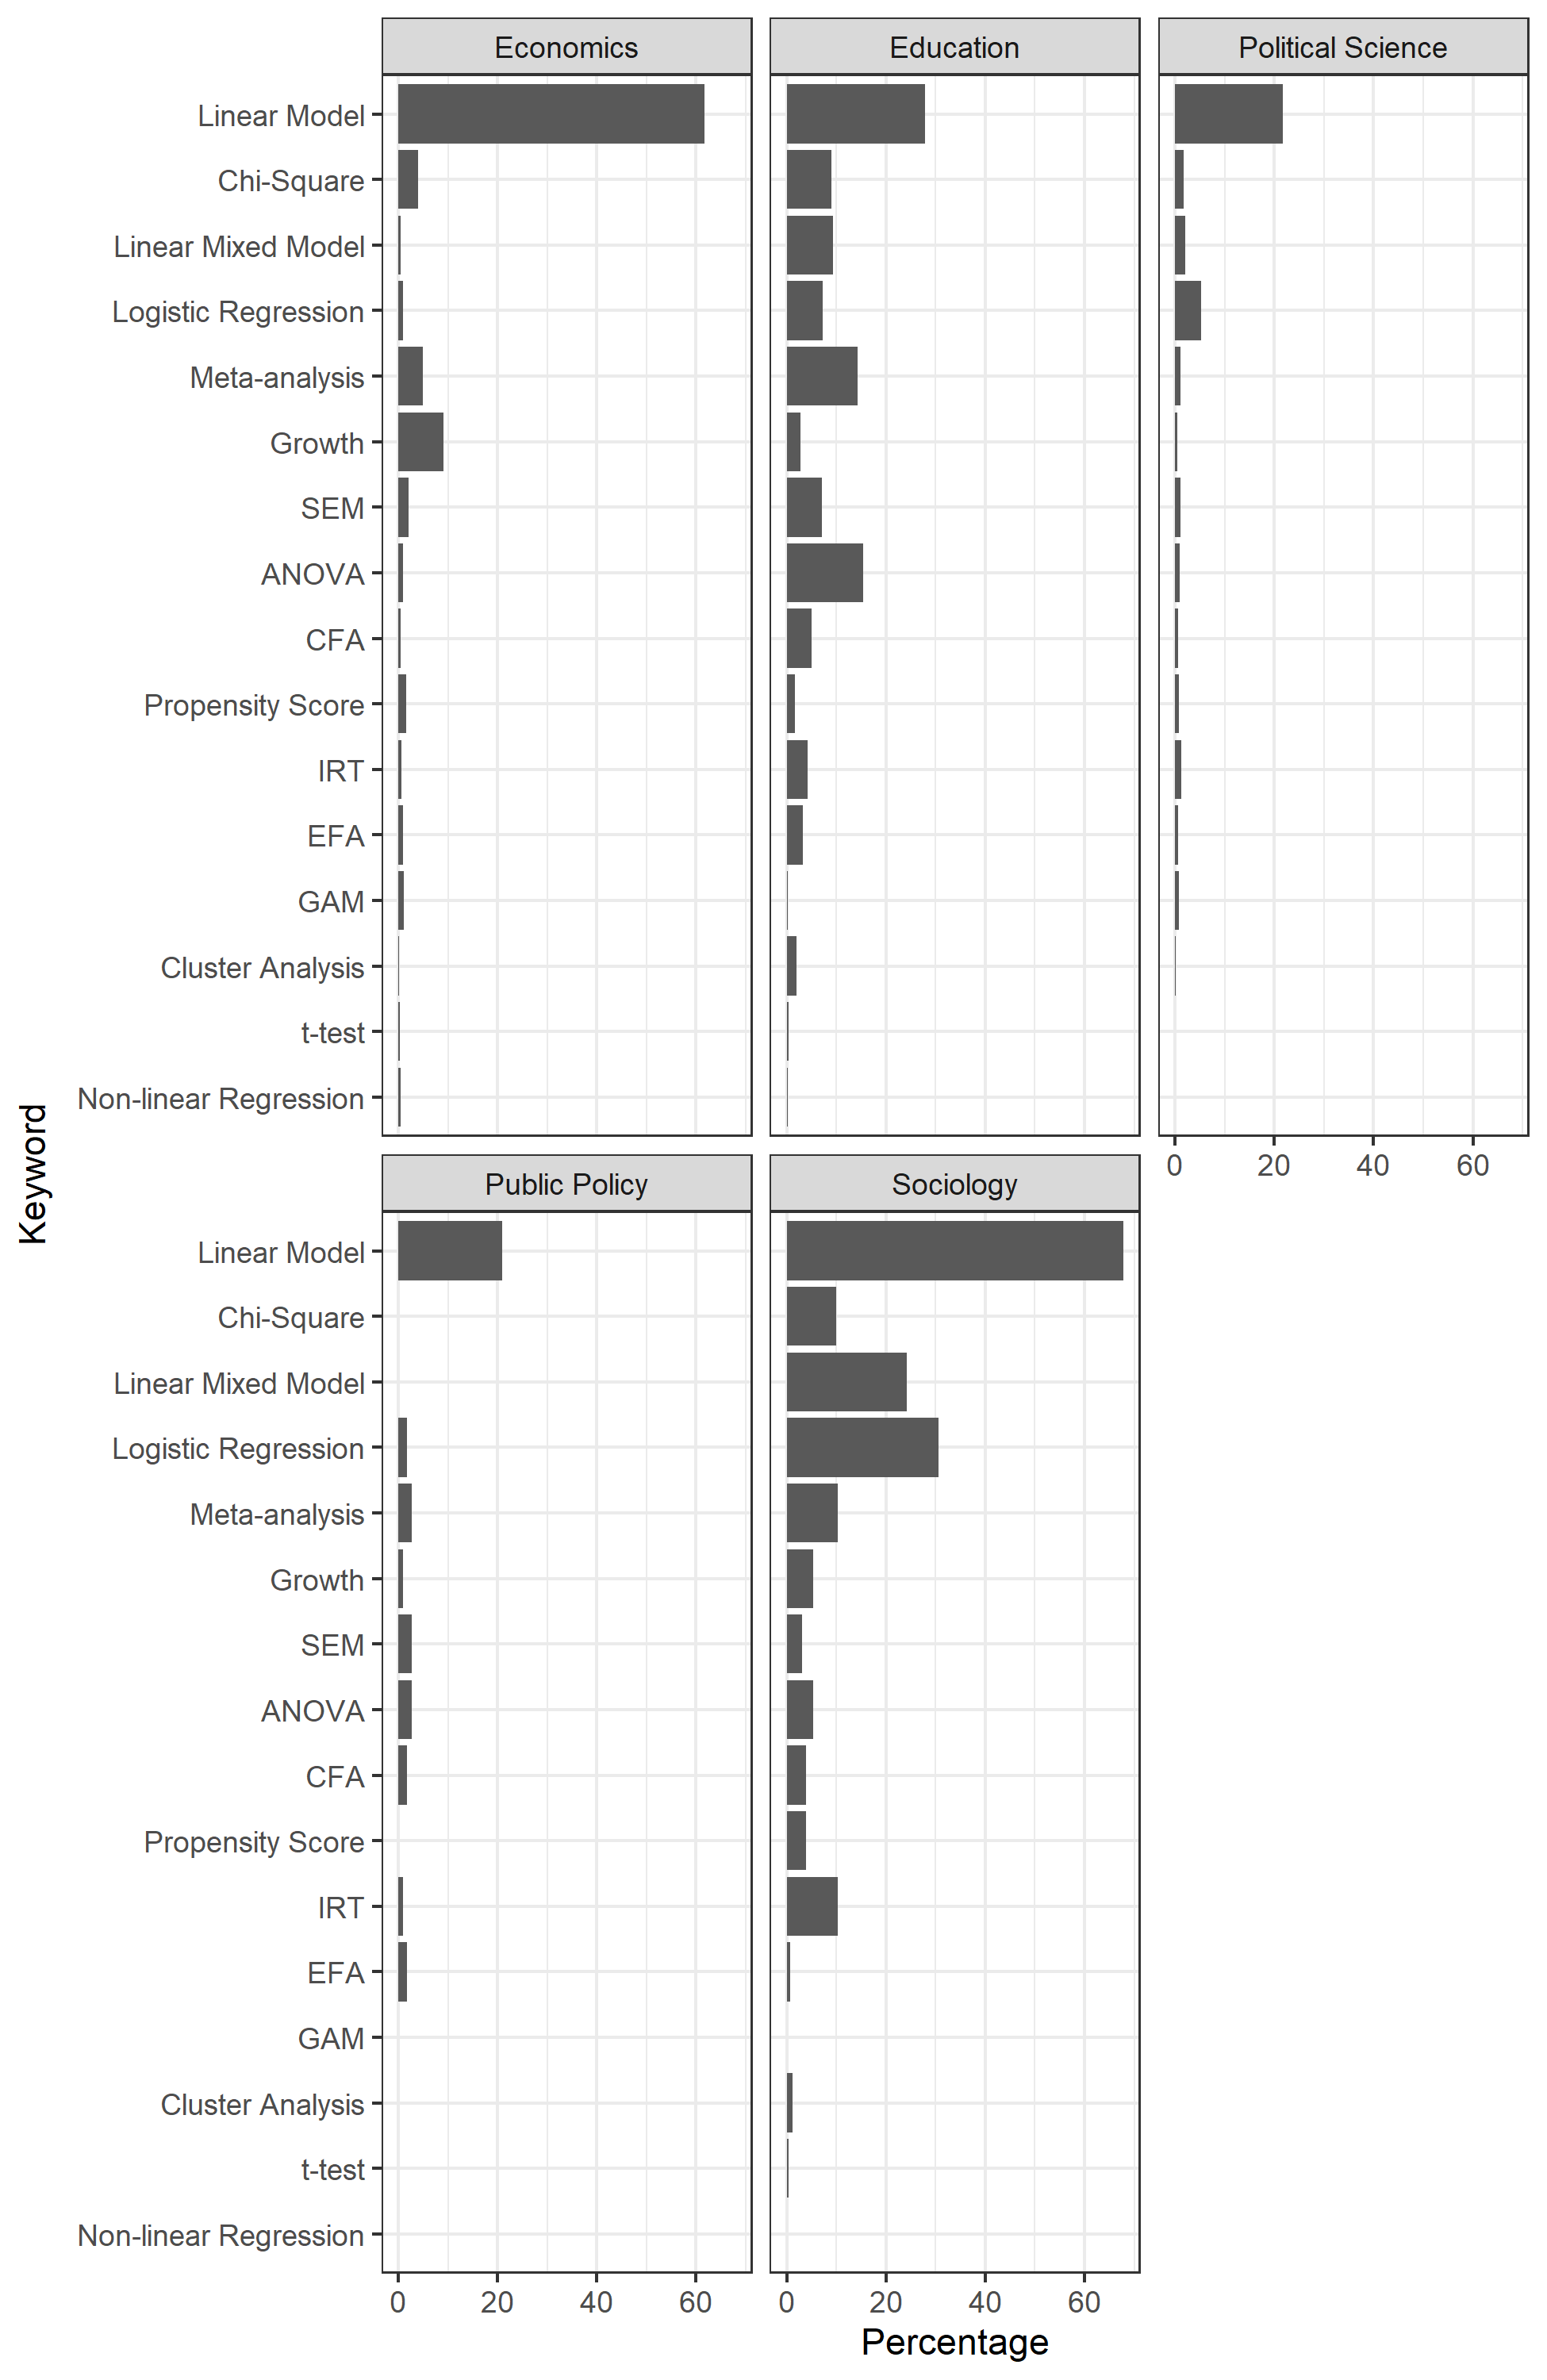
\includegraphics{software_files/figure-latex/model-discipline-1.pdf}
\caption{\label{fig:model-discipline}Statistical analysis counts by journal discipline}
\end{figure}

\hypertarget{impact-of-publication-year-on-keyword-rates}{%
\subsection{Impact of publication year on keyword rates}\label{impact-of-publication-year-on-keyword-rates}}

The impact of publication year on prevalence of software and analysis keywords within education were explored in Figures \ref{fig:software-year-at1} and \ref{fig:model-year-at1} for common software and analysis keywords respectively. In general, publication year does not have a strong impact on the software keyword rates with most trajectories being flat, on average, across the publication years. There was evidence that the percentage of articles having matching software keywords was unstable across years. R was consistently the most found software keyword and STATA was found the least across these publication years for education, but overall software was infrequently cited (see Figure \ref{fig:software-discipline}).

Commonly used specialty software in education, such as AMOS, HLM, LISREL, or Mplus, are shown in the bottom-most plot of Figure \ref{fig:software-year-at1}. Not surprisingly, the specialty software on average shows up less frequently compared to the general purpose software shown in the top-most plot of Figure \ref{fig:software-year-at1}. Out of these four specialty software, AMOS and LISREL showed up more frequently early in the published research obtained and have stayed relatively stable in the percentage of matches found. Mplus has gained additional usage over time and HLM software tended to show up infrequently, but has had a few years that the software showed up more than 15\%. However, these programs still only account for around 10\% or less of statistical software used in most years.

The usage of analysis keywords in education occurs more frequently and shows evidence of trends across publication years as shown in Figure \ref{fig:model-year-at1}. For example, the top figure shows a large increase in the prevalence of terms related to linear models (i.e.~regression models) or linear mixed models and shows a decline in analysis of variance methods. Logistic regression and the variety of t-tests are rarely mentioned in the articles included. The bottom figure also shows general increases in the four models depicted, particularly the mention of IRT and SEM methods. These two methods have gone from about 5\% of articles mentioning these terms in 1995 up to over 20\% in 2018. These gains are more modest compared to the increase in the mention of linear models from the top figure, but the increase has now put IRT and SEM methods about the same percentage as ANOVA and linear mixed models from the top figure.

\hypertarget{interaction-between-software-and-statistical-methods}{%
\subsection{Interaction between software and statistical methods}\label{interaction-between-software-and-statistical-methods}}

Figure \ref{fig:software-statmethods} shows a tile plot of the interaction between software (x-axis) and analysis (y-axis) keywords for education journals. The darker shaded regions of the figure show more combinations of the software and analysis keywords that were found within a single published manuscript For example, for a study to show up in the R and ANOVA tile of the plot, the study would need to mention both R and ANOVA in the manuscript. Darker colors would indicate more studies mentioning both of the keywords within the manuscript. In the figure, publication year is ignored to identify which methods are most closely paired with specific software; publication year will be explored separately in another figure. There are duplicates in the data for this figure, for example, an article may cite both R and SAS within the document and mentioned using a linear model. In this case, this article will show up in the R/linear model cell as well as the SAS/linear model cell. Any duplicate keyword combinations would only occur once for each article. This analysis is also limited to articles that have both a software and analysis keyword returned. On average, only about 20\% of all the PDFs obtained from the study in education journals had both a software and analysis keyword in them. This provides further evidence of the reporting bias, particularly with regard to software.

The figure shows that the most common combinations are R, SAS, and SPSS combined with linear model and ANOVA analysis keywords. AMOS, LISREL, and Mplus were most often mentioned with analysis keywords such as CFA, SEM, and chi-square, which are terms associated with latent variable models. Linear mixed models were most commonly used in HLM, R, and SAS. Meta-analysis is most commonly associated with R, SAS, and SPSS. In general, IRT specific software and STATA have evidence of not being mentioned much in the sampled studies.

The impact of publication year is explored next for the three general purpose statistical software found to be used frequently in education, R, SAS, and SPSS. Each panel in Figure \ref{fig:software-statmethods-year} represents a different publication year. In the panel label the percentage of articles that are missing are reported. More specifically, these are studies in which a PDF document was obtained but did not include at least one software keyword and at least one analysis keyword. These values range from a low of 70\% of the articles not appearing to a high of about 96\%. The percentage of missing articles starts out lower, increases, then decreases in more recent years. In general, however, there is evidence that many articles do not include both a software and analysis keyword.

The tile plot shown in Figure \ref{fig:software-statmethods-year} shows an increase in the percentage of keyword combinations that are found as the publications become more recent. This is shown by the figure filling in with light gray, as areas that are white indicate that no combination was found in the education articles sampled. There does not appear to be any significant trends over time with regard to which analyses are used in particular software, but there were articles using R, SAS, and SPSS with most of the statistical methods shown in Figure \ref{fig:software-statmethods-year} which supports the general usage of the software across a variety of analysis situations.

\hypertarget{discussion}{%
\section{Discussion}\label{discussion}}

This study explored the usage of statistical software and statistical analysis in published research from 1995 to 2018 across five education and a total of 12 social science journals. The journals that were selected were identified as journals within sub-fields of social science that were focused on publishing applied research spanning economics, education, political science, public policy, and sociology. After obtaining PDF documents from these journals, keyword searching was performed to extract keywords associated with statistical software and statistical methods (see Table \ref{tab:searchwords} for a list of search words that were used).

The results showed that statistical software keywords were not found as frequently as the statistical methods that are used to analyze the data. This has important implications for the reproducibility and replicability of the research that is being performed (Peng, 2009; Stodden et al., 2013). There has been an increase in the prevalence of software citations in published research, however the percentage of studies that cite software is still only about 20\% as of 2018. Evidence support differential software citations rates by journal and there was also evidence of specific statistical methods being used within journals. For example, JEE had evidence of stronger citation rates of statistical software and statistical methods keywords searched for.

There was also evidence of differences across disciplines. Sociology had the highest percentage of studies citing statistical software and methods keywords searched for in this study. Education had the second highest rate of software keywords found (21\%), but was not nearly as strong in the statistical methods keywords found with only about 27\% of studies containing a statistical method. Economics had evidence of more statistical methods found than education and education was similar to political science and public policy. It is unclear the exact reason why education has lower statistical method keywords found and would warrant more research. This small difference may be a reflection of the journals we chose, as there was evidence of JEE having more mention of statistical methods than any other journal included in the sample (see Figure \ref{fig:count-software}). Two education journals, Educational Researcher and Higher Education, have evidence of not publishing as much quantitative research (or at least these articles tend not to discuss the statistical method used), which is decreasing the education percentages reported. It may also be that education has more qualitative studies which was not searched for in the current study.

Publication year did not have a large impact on which software is being used in published research and there is evidence that the software is highly variable across years. This may be due to the small sample of studies that actually do include information about the statistical software used. With only a small number of studies in a publication year, the percentage citing software can vary widely with only a few additional mentions in a single year. More stable estimates across a wider variety of journals would be a natural extension to this research, including the exploration of open-access and other education or social science journals that do not have as large of an impact factor.

The statistical software, R, had evidence of being highly cited compared to other statistical software over time. Although the publication year didn't show much difference in how often R is being cited, a finding that differs from Muenchen (2017). The differences may be due to the different methodology where Muenchen (2017) is sampling all manuscripts indexed by Google Scholar whereas this study is more focused on higher impact journals in social science disciplines. The high citation rate found in this study for R may be due to R users being more motivated to cite the software or due to R providing a citation function that makes it easy to generate R and R package citations (i.e.~the \texttt{citation()} function can be used for this). This is anecdotal evidence that would warrant additional exploration. There also could be users following the APA guidelines for not needing to cite general purpose statistical software, a practice that we do not recommend following. SPSS had evidence of showing up frequently in education, an observation found by Muenchen (2017).

\hypertarget{recommendations-for-practice}{%
\subsection{Recommendations for Practice}\label{recommendations-for-practice}}

This study provides evidence that statistical software is not commonly cited in published research. Without appropriate statistical software citations, it can be much more difficult for others to replicate or reproduce the work of other studies. In addition, when differences are found, it would be unclear if the differences are due to the unreplicability of the findings or due to differences in statistical software specifications. For example, default settings across general purpose or specialized statistical software could explain differences in study results.

We want to promote the citation of statistical software along with the statistical methods being used. Statistical software takes time to implement, test, evaluate, and release; therefore, users of this software should cite the software used to acknowledge the time developers have spent. Statistical software is also a strong contribution to the field that enables many researchers to conduct their own work and citations of the software is one way to promote that impact. If more statistical software is cited, the transparency and reproducibility of studies will be increased as well, another benefit of citing the software used in the research. However, the citation of statistical software is not enough, the specific version used and operating system used is also needed as implementations evolve, software bugs are fixed, and default settings can change over time. Software citations are a necessary but not a sufficient condition to ensure proper transparency and reproducibility of study results.

\hypertarget{future-research}{%
\subsection{Future Research}\label{future-research}}

This study explored, through extraction of text from within the published research documents, the identification of statistical software and statistical methods used. It may be possible, either through supplemental materials, an Open Science Framework page, GitHub repository, Zenodo repository, or other sources in which the statistical code is openly shared. These resources could be a further source of information on which statistical software and statistical methods were used, even if they were not directly cited or mentioned in the published document. Preprints could be another source of information that could contain additional information as published articles in traditional journals that often have page or word limits that may limit space for inclusion of specific details about software or methods.

\newpage

\begin{figure}
\centering
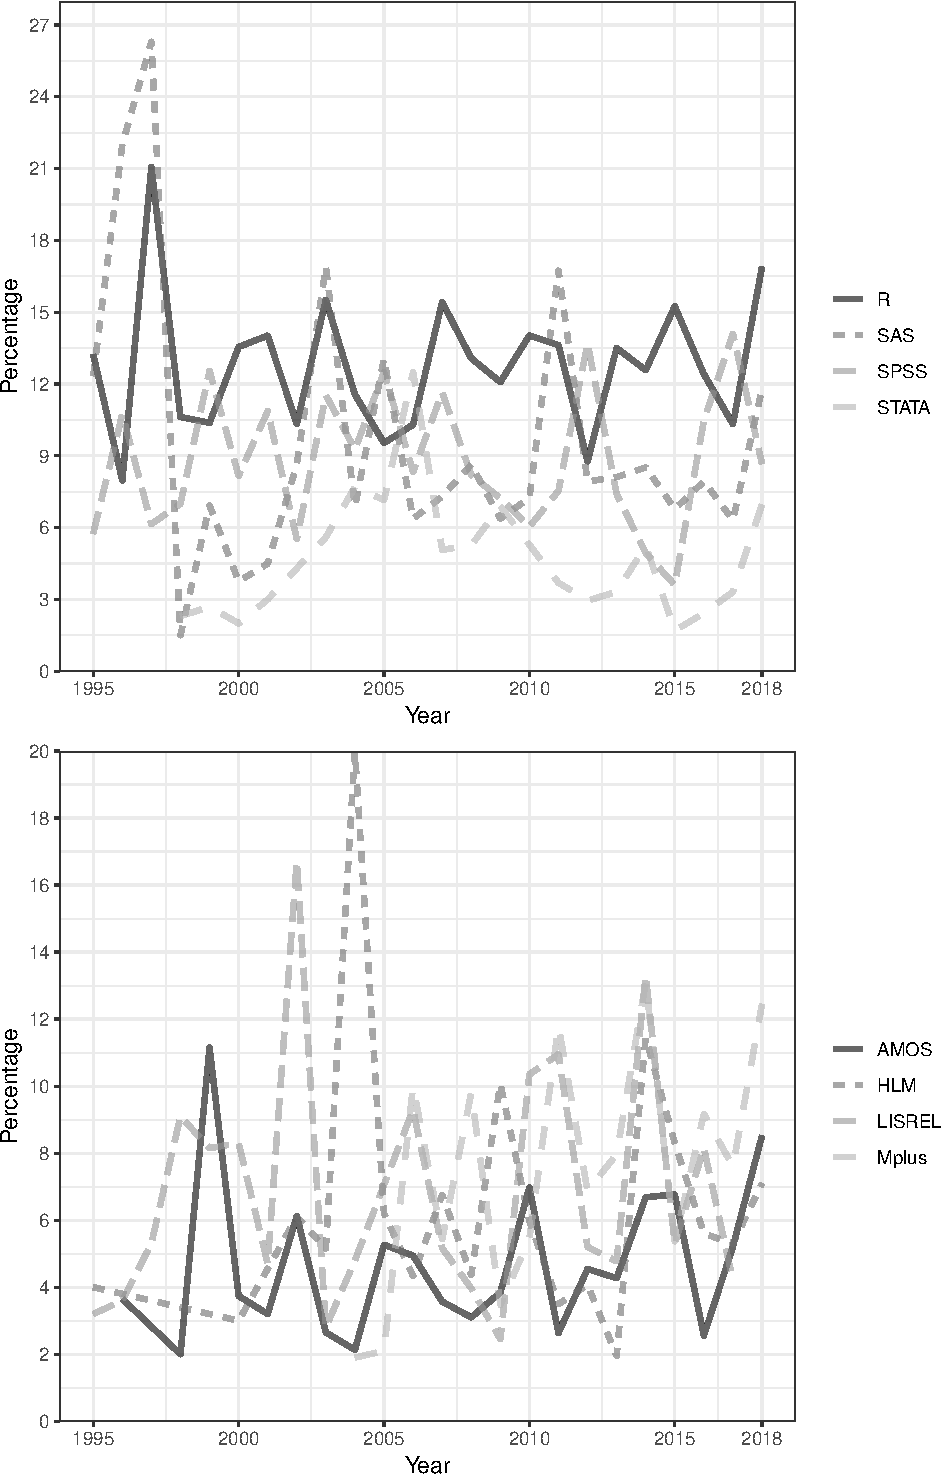
\includegraphics{software_files/figure-latex/software-year-at1-1.pdf}
\caption{\label{fig:software-year-at1}Software percentages by year for education journals}
\end{figure}

\begin{figure}
\centering
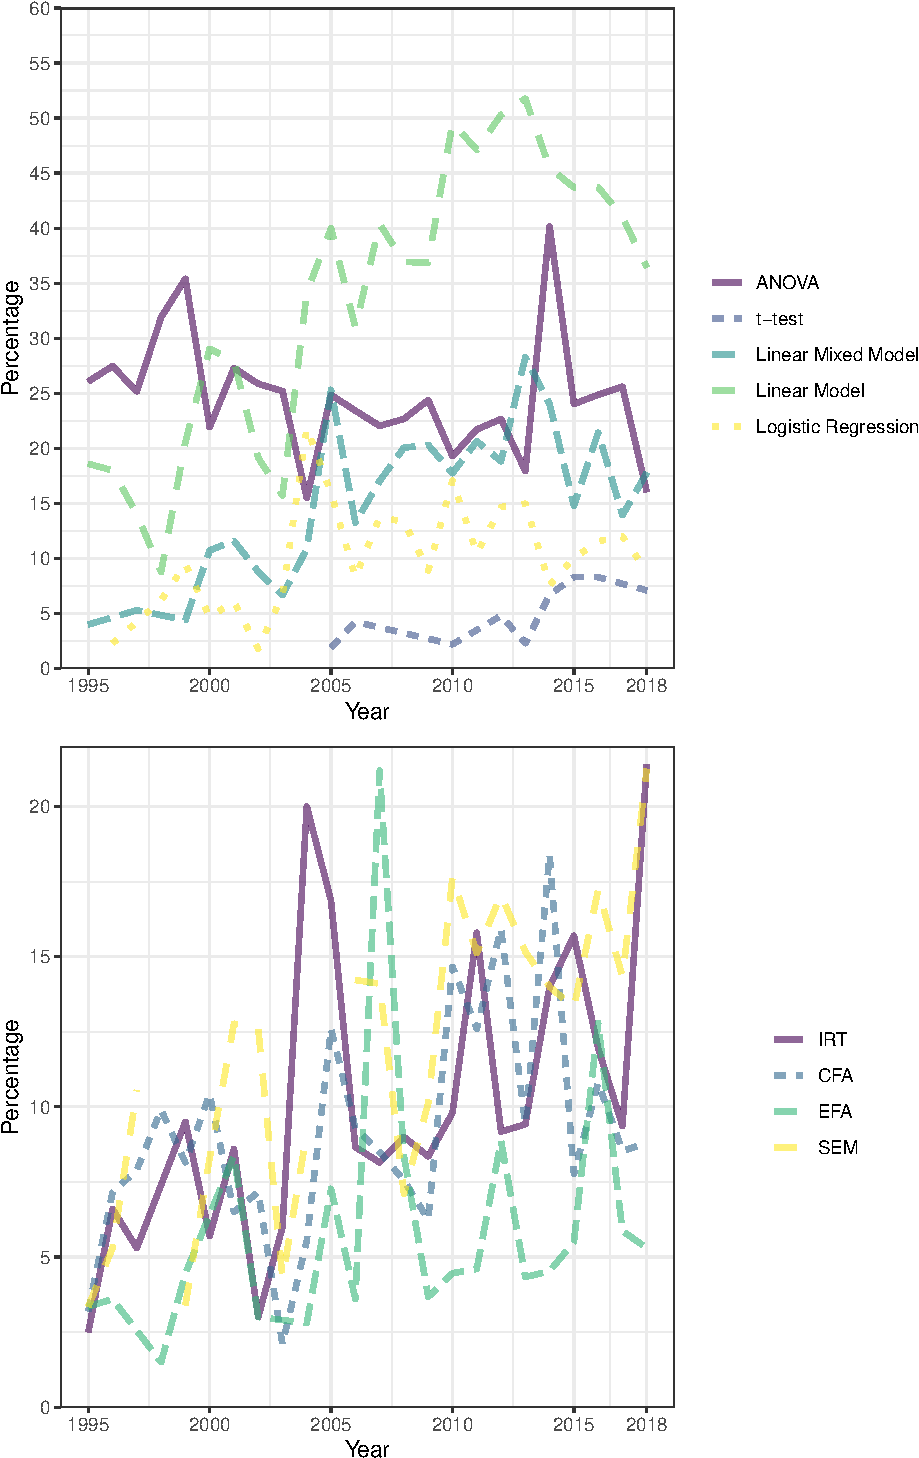
\includegraphics{software_files/figure-latex/model-year-at1-1.pdf}
\caption{\label{fig:model-year-at1}Percentages by year for education journals by statistical analysis}
\end{figure}

\begin{figure}
\centering
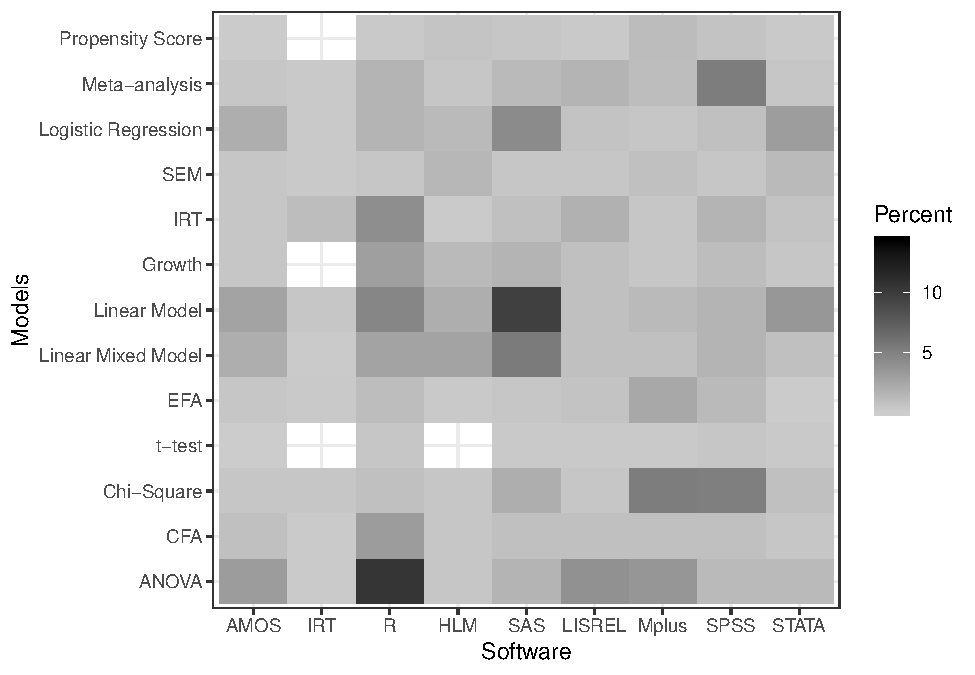
\includegraphics{software_files/figure-latex/software-statmethods-1.pdf}
\caption{\label{fig:software-statmethods}Tile plot showing interaction between software and statistical methods for education journals.}
\end{figure}

\begin{figure}
\centering
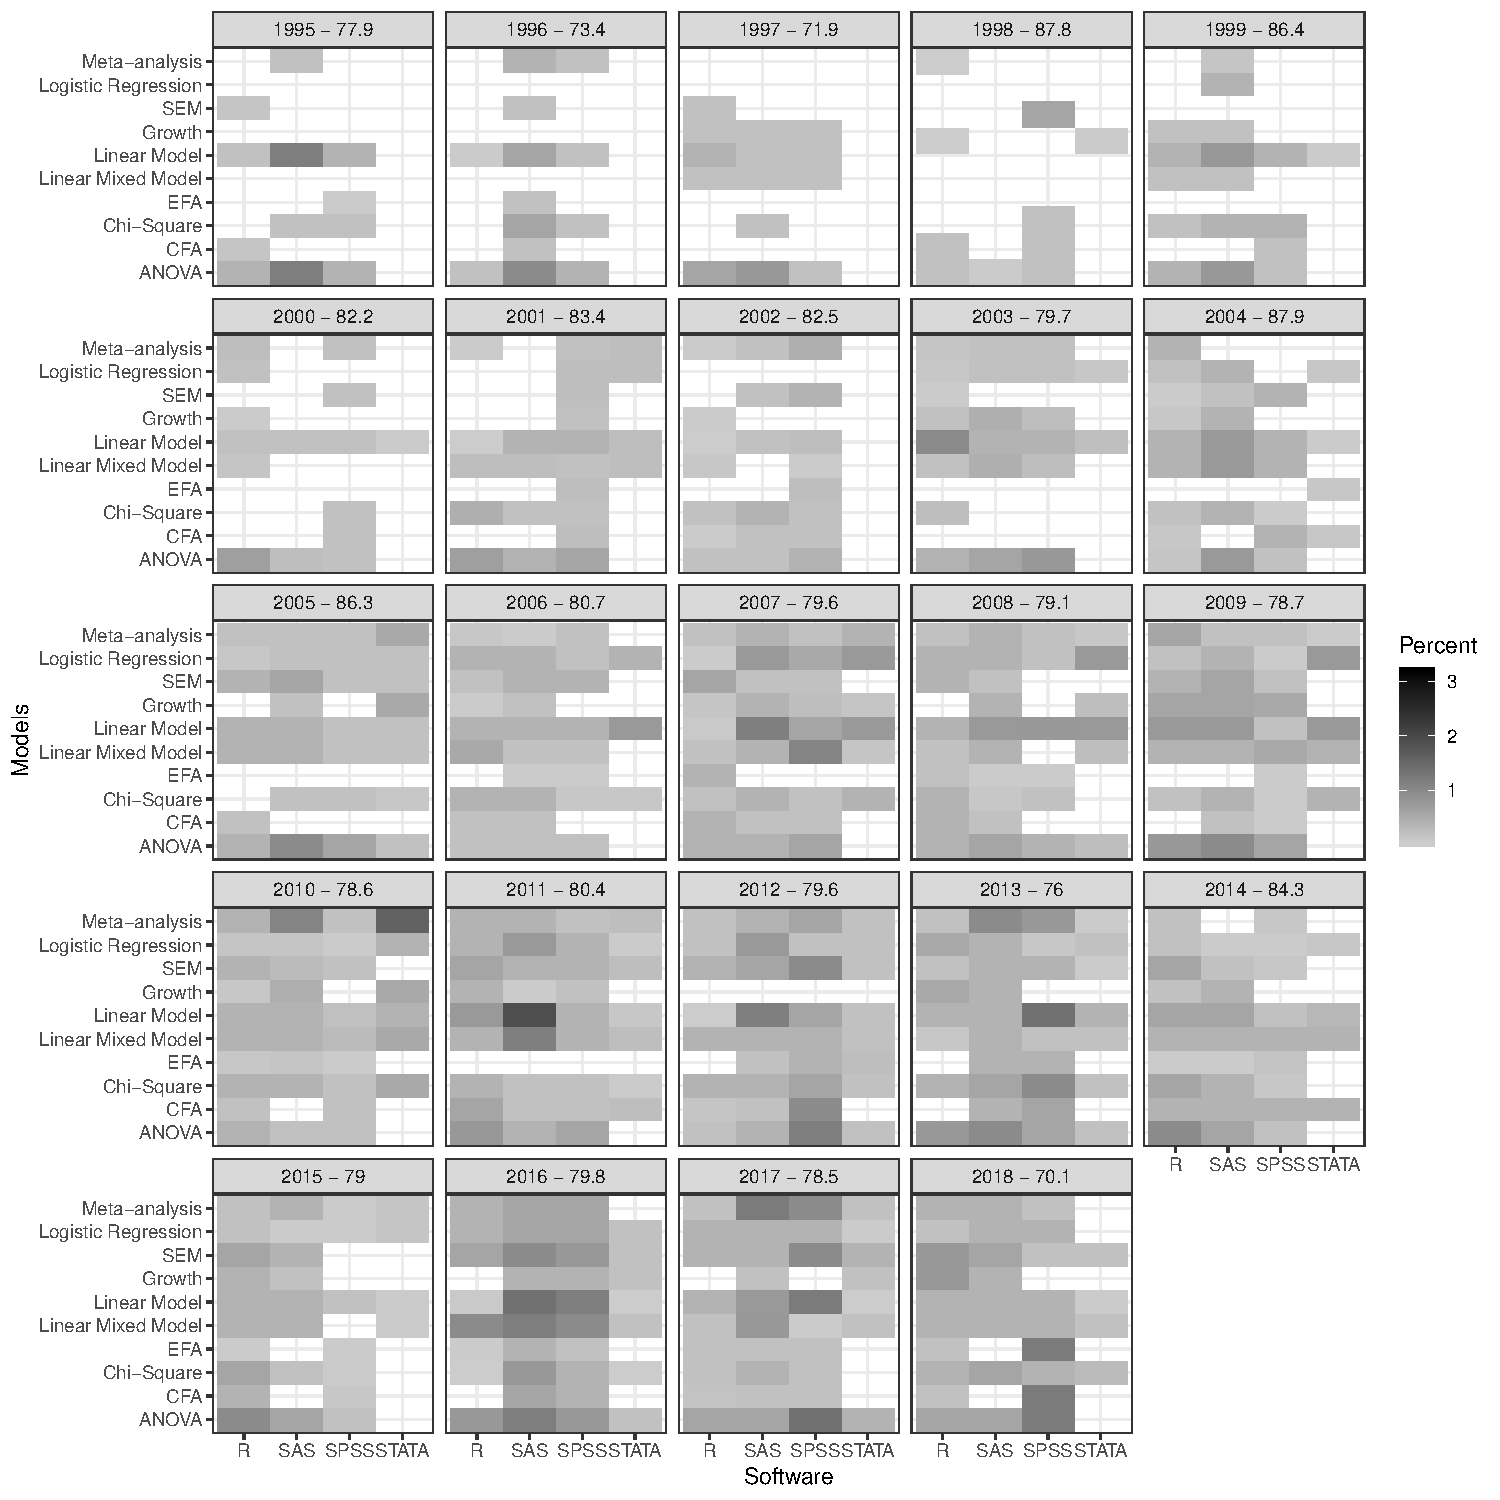
\includegraphics{software_files/figure-latex/software-statmethods-year-1.pdf}
\caption{\label{fig:software-statmethods-year}Tile plot showing interaction between software and statistical methods by publication year for primary software in education journals.}
\end{figure}

\newpage

\hypertarget{references}{%
\section{References}\label{references}}

\setlength{\parindent}{-0.5in}
\setlength{\leftskip}{0.5in}

\hypertarget{refs}{}
\begin{cslreferences}
\leavevmode\hypertarget{ref-rmarkdown}{}%
Allaire, J., Cheng, J., Xie, Y., McPherson, J., Chang, W., Allen, J., \ldots{} Arslan, R. (2017). \emph{Rmarkdown: Dynamic documents for r}. Retrieved from \url{https://CRAN.R-project.org/package=rmarkdown}

\leavevmode\hypertarget{ref-apa}{}%
American Psychological Association. (2010). \emph{Publication manual of the american psychological association}. Washington, D.C.: American Psychological Association.

\leavevmode\hypertarget{ref-asendorpf2013}{}%
Asendorpf, J. B., Conner, M., De Fruyt, F., De Houwer, J., Denissen, J. J., Fiedler, K., \ldots{} others. (2013). Recommendations for increasing replicability in psychology. \emph{European Journal of Personality}, \emph{27}(2), 108--119.

\leavevmode\hypertarget{ref-cooper2016}{}%
Cooper, H. (2016). \emph{Research synthesis and meta-analysis: A step-by-step approach} (Vol. 2). Sage publications.

\leavevmode\hypertarget{ref-hedges2019}{}%
Hedges, L. V., \& Schauer, J. M. (2019). More than one replication study is needed for unambiguous tests of replication. \emph{Journal of Educational and Behavioral Statistics}, 1076998619852953.

\leavevmode\hypertarget{ref-hendrick1990}{}%
Hendrick, C. (1990). Replications, strict replications, and conceptual replications: Are they important? \emph{Journal of Social Behavior and Personality}, \emph{5}(4), 41.

\leavevmode\hypertarget{ref-spss}{}%
IBM Corp. (2019). \emph{IBM SPSS Statistics}. Armonk, NY: IBM Corp.

\leavevmode\hypertarget{ref-iesdata}{}%
Insitute of Education Sciences (IES), U.S. Department of Education. (2018). Resources for researchers: Policy statement on public access to data resulting from ies funded grants. Retrieved from \url{https://ies.ed.gov/funding/datasharing_policy.asp}

\leavevmode\hypertarget{ref-iesrepro}{}%
Insitute of Education Sciences (IES), U.S. Department of Education and National Science Foundation (NSF). (2018). Companion guidelines on replication \& reproducibility in education research: A supplement to the common guidelines for education reserach and development. Retrieved from \url{https://ies.ed.gov/pdf/CompanionGuidelinesReplicationReproducibility.pdf}

\leavevmode\hypertarget{ref-ioannidis2014}{}%
Ioannidis, J. P. (2014). How to make more published research true. \emph{PLoS Medicine}, \emph{11}(10), e1001747.

\leavevmode\hypertarget{ref-iqbal2016}{}%
Iqbal, S. A., Wallach, J. D., Khoury, M. J., Schully, S. D., \& Ioannidis, J. P. (2016). Reproducible research practices and transparency across the biomedical literature. \emph{PLoS Biology}, \emph{14}(1), e1002333.

\leavevmode\hypertarget{ref-kluyver2016}{}%
Kluyver, T., Ragan-Kelley, B., Pérez, F., Granger, B., Bussonnier, M., Frederic, J., \ldots{} Willing, C. (2016). Jupyter notebooks -- a publishing format for reproducible computational workflows. (F. Loizides \& B. Schmidt, Eds.). IOS Press.

\leavevmode\hypertarget{ref-pdfsearch}{}%
LeBeau, B. (2018). pdfsearch: Search tools for pdf files. \emph{Journal of Open Source Software}, \emph{3}(27), 668. doi:\href{https://doi.org/10.21105/joss.00668}{10.21105/joss.00668}

\leavevmode\hypertarget{ref-makel2014}{}%
Makel, M. C., \& Plucker, J. A. (2014). Facts are more important than novelty: Replication in the education sciences. \emph{Educational Researcher}, \emph{43}(6), 304--316.

\leavevmode\hypertarget{ref-makel2012}{}%
Makel, M. C., Plucker, J. A., \& Hegarty, B. (2012). Replications in psychology research: How often do they really occur? \emph{Perspectives on Psychological Science}, \emph{7}(6), 537--542.

\leavevmode\hypertarget{ref-makel2019path}{}%
Makel, M. C., Smith, K. N., McBee, M. T., Peters, S. J., \& Miller, E. M. (2019). A path to greater credibility: Large-scale collaborative education research. \emph{AERA Open}, \emph{5}(4), 2332858419891963.

\leavevmode\hypertarget{ref-mcbee2018call}{}%
McBee, M. T., Makel, M. C., Peters, S. J., \& Matthews, M. S. (2018). A call for open science in giftedness research. \emph{Gifted Child Quarterly}, \emph{62}(4), 374--388.

\leavevmode\hypertarget{ref-miguel2014}{}%
Miguel, E., Camerer, C., Casey, K., Cohen, J., Esterling, K. M., Gerber, A., \ldots{} others. (2014). Promoting transparency in social science research. \emph{Science}, \emph{343}(6166), 30--31.

\leavevmode\hypertarget{ref-muenchen}{}%
Muenchen, R. A. (2017). The popularity of data science software. Retrieved from \url{http://r4stats.com/articles/popularity/}

\leavevmode\hypertarget{ref-bib2df}{}%
Ottolinger, P. (2018). \emph{Bib2df: Parse a bibtex file to a data.frame}. Retrieved from \url{https://CRAN.R-project.org/package=bib2df}

\leavevmode\hypertarget{ref-peng2009}{}%
Peng, R. D. (2009). Reproducible research and biostatistics. \emph{Biostatistics}, \emph{10}(3), 405--408. doi:\href{https://doi.org/10.1093/biostatistics/kxp014}{10.1093/biostatistics/kxp014}

\leavevmode\hypertarget{ref-peng2011}{}%
Peng, R. D. (2011). Reproducible research in computational science. \emph{Science}, \emph{334}(6060), 1226--1227.

\leavevmode\hypertarget{ref-rpro}{}%
R Core Team. (2019). \emph{R: A language and environment for statistical computing}. Vienna, Austria: R Foundation for Statistical Computing. Retrieved from \url{https://www.R-project.org/}

\leavevmode\hypertarget{ref-sas2017base}{}%
SAS Institute. (2017). \emph{Base sas 9.4 procedures guide: Statistical procedures}. SAS Institute.

\leavevmode\hypertarget{ref-schmidt2009}{}%
Schmidt, S. (2009). Shall we really do it again? The powerful concept of replication is neglected in the social sciences. \emph{Review of General Psychology}, \emph{13}(2), 90.

\leavevmode\hypertarget{ref-stata}{}%
StataCorp. (2019). \emph{Stata statistical software: Release 16}. College Station, TX: StataCrop LLC.

\leavevmode\hypertarget{ref-stodden2012}{}%
Stodden, V. (2012). Reproducible research for scientific computing: Tools and strategies for changing the culture. \emph{Computing in Science \& Engineering}, \emph{14}(4), 13--17.

\leavevmode\hypertarget{ref-stodden2013}{}%
Stodden, V., Miguez, S., LeVeque, R., Malm, H., Novitzky, P., \& Gordijn, B. (2013). Resolving irreproducibility in empirical and computational research. \emph{IMS Bulletin}, \emph{14}(4).

\leavevmode\hypertarget{ref-tatman2015}{}%
Tatman, R. (2015). The state of the stats: Current use of statistical methods across linguistics subfields. \emph{Linguistics Summer Institute}.

\leavevmode\hypertarget{ref-van1995python}{}%
Van Rossum, G., \& Drake Jr, F. L. (1995). \emph{Python tutorial}. Centrum voor Wiskunde en Informatica Amsterdam, The Netherlands.

\leavevmode\hypertarget{ref-ggplot2}{}%
Wickham, H. (2016). \emph{Ggplot2: Elegant graphics for data analysis}. Springer-Verlag New York. Retrieved from \url{http://ggplot2.org}

\leavevmode\hypertarget{ref-knitr}{}%
Xie, Y. (2015). \emph{Dynamic documents with R and knitr} (2nd ed.). Boca Raton, Florida: Chapman; Hall/CRC. Retrieved from \url{http://yihui.name/knitr/}

\leavevmode\hypertarget{ref-knitrmanual}{}%
Xie, Y. (2017). \emph{Knitr: A general-purpose package for dynamic report generation in r}. Retrieved from \url{http://yihui.name/knitr/}

\leavevmode\hypertarget{ref-rmarkdown}{}%
Allaire, J., Cheng, J., Xie, Y., McPherson, J., Chang, W., Allen, J., \ldots{} Arslan, R. (2017). \emph{Rmarkdown: Dynamic documents for r}. Retrieved from \url{https://CRAN.R-project.org/package=rmarkdown}

\leavevmode\hypertarget{ref-apa}{}%
American Psychological Association. (2010). \emph{Publication manual of the american psychological association}. Washington, D.C.: American Psychological Association.

\leavevmode\hypertarget{ref-asendorpf2013}{}%
Asendorpf, J. B., Conner, M., De Fruyt, F., De Houwer, J., Denissen, J. J., Fiedler, K., \ldots{} others. (2013). Recommendations for increasing replicability in psychology. \emph{European Journal of Personality}, \emph{27}(2), 108--119.

\leavevmode\hypertarget{ref-cooper2016}{}%
Cooper, H. (2016). \emph{Research synthesis and meta-analysis: A step-by-step approach} (Vol. 2). Sage publications.

\leavevmode\hypertarget{ref-hedges2019}{}%
Hedges, L. V., \& Schauer, J. M. (2019). More than one replication study is needed for unambiguous tests of replication. \emph{Journal of Educational and Behavioral Statistics}, 1076998619852953.

\leavevmode\hypertarget{ref-hendrick1990}{}%
Hendrick, C. (1990). Replications, strict replications, and conceptual replications: Are they important? \emph{Journal of Social Behavior and Personality}, \emph{5}(4), 41.

\leavevmode\hypertarget{ref-spss}{}%
IBM Corp. (2019). \emph{IBM SPSS Statistics}. Armonk, NY: IBM Corp.

\leavevmode\hypertarget{ref-iesdata}{}%
Insitute of Education Sciences (IES), U.S. Department of Education. (2018). Resources for researchers: Policy statement on public access to data resulting from ies funded grants. Retrieved from \url{https://ies.ed.gov/funding/datasharing_policy.asp}

\leavevmode\hypertarget{ref-iesrepro}{}%
Insitute of Education Sciences (IES), U.S. Department of Education and National Science Foundation (NSF). (2018). Companion guidelines on replication \& reproducibility in education research: A supplement to the common guidelines for education reserach and development. Retrieved from \url{https://ies.ed.gov/pdf/CompanionGuidelinesReplicationReproducibility.pdf}

\leavevmode\hypertarget{ref-ioannidis2014}{}%
Ioannidis, J. P. (2014). How to make more published research true. \emph{PLoS Medicine}, \emph{11}(10), e1001747.

\leavevmode\hypertarget{ref-iqbal2016}{}%
Iqbal, S. A., Wallach, J. D., Khoury, M. J., Schully, S. D., \& Ioannidis, J. P. (2016). Reproducible research practices and transparency across the biomedical literature. \emph{PLoS Biology}, \emph{14}(1), e1002333.

\leavevmode\hypertarget{ref-kluyver2016}{}%
Kluyver, T., Ragan-Kelley, B., Pérez, F., Granger, B., Bussonnier, M., Frederic, J., \ldots{} Willing, C. (2016). Jupyter notebooks -- a publishing format for reproducible computational workflows. (F. Loizides \& B. Schmidt, Eds.). IOS Press.

\leavevmode\hypertarget{ref-pdfsearch}{}%
LeBeau, B. (2018). pdfsearch: Search tools for pdf files. \emph{Journal of Open Source Software}, \emph{3}(27), 668. doi:\href{https://doi.org/10.21105/joss.00668}{10.21105/joss.00668}

\leavevmode\hypertarget{ref-makel2014}{}%
Makel, M. C., \& Plucker, J. A. (2014). Facts are more important than novelty: Replication in the education sciences. \emph{Educational Researcher}, \emph{43}(6), 304--316.

\leavevmode\hypertarget{ref-makel2012}{}%
Makel, M. C., Plucker, J. A., \& Hegarty, B. (2012). Replications in psychology research: How often do they really occur? \emph{Perspectives on Psychological Science}, \emph{7}(6), 537--542.

\leavevmode\hypertarget{ref-makel2019path}{}%
Makel, M. C., Smith, K. N., McBee, M. T., Peters, S. J., \& Miller, E. M. (2019). A path to greater credibility: Large-scale collaborative education research. \emph{AERA Open}, \emph{5}(4), 2332858419891963.

\leavevmode\hypertarget{ref-mcbee2018call}{}%
McBee, M. T., Makel, M. C., Peters, S. J., \& Matthews, M. S. (2018). A call for open science in giftedness research. \emph{Gifted Child Quarterly}, \emph{62}(4), 374--388.

\leavevmode\hypertarget{ref-miguel2014}{}%
Miguel, E., Camerer, C., Casey, K., Cohen, J., Esterling, K. M., Gerber, A., \ldots{} others. (2014). Promoting transparency in social science research. \emph{Science}, \emph{343}(6166), 30--31.

\leavevmode\hypertarget{ref-muenchen}{}%
Muenchen, R. A. (2017). The popularity of data science software. Retrieved from \url{http://r4stats.com/articles/popularity/}

\leavevmode\hypertarget{ref-bib2df}{}%
Ottolinger, P. (2018). \emph{Bib2df: Parse a bibtex file to a data.frame}. Retrieved from \url{https://CRAN.R-project.org/package=bib2df}

\leavevmode\hypertarget{ref-peng2009}{}%
Peng, R. D. (2009). Reproducible research and biostatistics. \emph{Biostatistics}, \emph{10}(3), 405--408. doi:\href{https://doi.org/10.1093/biostatistics/kxp014}{10.1093/biostatistics/kxp014}

\leavevmode\hypertarget{ref-peng2011}{}%
Peng, R. D. (2011). Reproducible research in computational science. \emph{Science}, \emph{334}(6060), 1226--1227.

\leavevmode\hypertarget{ref-rpro}{}%
R Core Team. (2019). \emph{R: A language and environment for statistical computing}. Vienna, Austria: R Foundation for Statistical Computing. Retrieved from \url{https://www.R-project.org/}

\leavevmode\hypertarget{ref-sas2017base}{}%
SAS Institute. (2017). \emph{Base sas 9.4 procedures guide: Statistical procedures}. SAS Institute.

\leavevmode\hypertarget{ref-schmidt2009}{}%
Schmidt, S. (2009). Shall we really do it again? The powerful concept of replication is neglected in the social sciences. \emph{Review of General Psychology}, \emph{13}(2), 90.

\leavevmode\hypertarget{ref-stata}{}%
StataCorp. (2019). \emph{Stata statistical software: Release 16}. College Station, TX: StataCrop LLC.

\leavevmode\hypertarget{ref-stodden2012}{}%
Stodden, V. (2012). Reproducible research for scientific computing: Tools and strategies for changing the culture. \emph{Computing in Science \& Engineering}, \emph{14}(4), 13--17.

\leavevmode\hypertarget{ref-stodden2013}{}%
Stodden, V., Miguez, S., LeVeque, R., Malm, H., Novitzky, P., \& Gordijn, B. (2013). Resolving irreproducibility in empirical and computational research. \emph{IMS Bulletin}, \emph{14}(4).

\leavevmode\hypertarget{ref-tatman2015}{}%
Tatman, R. (2015). The state of the stats: Current use of statistical methods across linguistics subfields. \emph{Linguistics Summer Institute}.

\leavevmode\hypertarget{ref-van1995python}{}%
Van Rossum, G., \& Drake Jr, F. L. (1995). \emph{Python tutorial}. Centrum voor Wiskunde en Informatica Amsterdam, The Netherlands.

\leavevmode\hypertarget{ref-ggplot2}{}%
Wickham, H. (2016). \emph{Ggplot2: Elegant graphics for data analysis}. Springer-Verlag New York. Retrieved from \url{http://ggplot2.org}

\leavevmode\hypertarget{ref-knitr}{}%
Xie, Y. (2015). \emph{Dynamic documents with R and knitr} (2nd ed.). Boca Raton, Florida: Chapman; Hall/CRC. Retrieved from \url{http://yihui.name/knitr/}

\leavevmode\hypertarget{ref-knitrmanual}{}%
Xie, Y. (2017). \emph{Knitr: A general-purpose package for dynamic report generation in r}. Retrieved from \url{http://yihui.name/knitr/}
\end{cslreferences}

\end{document}
